\section{Kupfer-PVD}
\label{copperpvd}

Mit Kupfer-PVD wurde ein zweiter Metall-PVD-Prozess auf Parsivald angepasst und unter der Zielsetzung simuliert, die Anwendbarkeit verschiedener Potentialparametrisierungen zu prüfen.
Der Prozess ähnelt dem Gold-Prozess in seinen Parametern, jedoch konnten viele verschiedene Parametersätze für Kupferoberflächen, -schmelzen und  und -legierungen gefunden werden, von denen einige Hinweise auf die Nicht-Darstellbarkeit der reinen Metallsysteme enthalten\cite{mendelev_development_2009}\cite{mendelev_using_2007}.

\begin{table}
  \caption[EAM-Parametrisierungen für Kupfersysteme]{EAM-Parametrisierungen für Kupfersysteme.}
  \label{tab:copperpots}
  \rowcolors{0}{white}{lightgray}
  \begin{tabularx}{\textwidth}{|lXc|}
    \hline
    \textbf{Bezeichnung} & \textbf{Anwendung \& Kommentare} & \textbf{Ref.} \\
    \hline
    CuAg.eam.alloy & Strukturelle und thermodynamische Eigenschaften von \ce{Cu-Ag} & \cite{williams_embedded-atom_2006} \\
    cu\_ag\_ymwu.eam.alloy & Mono-, Di-, Trimere und Inseln von \ce{Cu} auf \ce{Ag} & \cite{wu_cu/ag_2009} \\
    Cu\_smf7.eam & Oberflächen von \ce{Ni-Cu}-Legierungen bei \SI{800}{\kelvin} & \cite{foiles_calculation_1985} \\
    Cu\_u3.eam & Oberflächen und Bulks verschiedener Legierungen & \cite{foiles_embedded-atom-method_1986} \\
    Cu\_u6.eam & Aktivierungsenergie für Eigendiffusionen & \cite{adams_self-diffusion_1989} \\
    Cu-Zr\_2.eam.fs & Flüssige und amorphe \ce{Cu-Zr}-Legierungen & \cite{mendelev_development_2009} \\
    Cu-Zr.eam.fs & Flüssige und amorphe \ce{Cu-Zr}-Legierungen & \cite{mendelev_using_2007} \\
    Mendelev\_Cu2\_2012.eam.fs & Unterkühlte \ce{Al-Cu}-Schmelzen. Basiert auf \cite{mendelev_analysis_2008} & \cite{_interatomic_2014} \\
    \hline
  \end{tabularx}
  
\end{table}

\subsection{Voruntersuchungen}

\todo[inline]{fuckfuckfuck! habe den falschen pair\_style benutzt!}
Die drei Parametersätze Cu\_u3.eam, Cu\_u6.eam und Cu\_smf7.eam wurden die Parameterdateien nicht von LAMMPS akzeptiert.
Es zeigten sich Probleme beim Laden der Dateien, kryptische Fehlerausgaben nach wenigen Schritten oder ein Aufhängen der Simulation ohne Vorankündigung.\todo{Ursachensuche?}
Die Ergebnisse der verbliebenen Simulationen zeigen aber gute Übereinstimmung mit Literaturwerten (Tabelle \ref{tab:copperpreresults}).
Einzig der Schmelzpunkt wird stark überschätzt (Abbildung \ref{fig:copperthermo}), was durch üblicherweise geringe Simulationstemperaturen vernachlässigbar ist.

\begin{table}
  \rowcolors{0}{white}{lightgray} 
  \caption[Eigenschaften von Kupfer]{Voruntersuchungen: Vergleich der Simulationsergebnisse mit Literaturdaten}
  \label{tab:copperpreresults}
  \begin{tabularx}{\textwidth}{|Xrrr|}
    \hline
    \textbf{Parametersatz}  &  \textbf{Koord.}  &  \textbf{Bindungslänge}                        &  \textbf{Dichte}                            \\
    \hline
    \textbf{Experiment}     &  \num{12.00}      &  \SI{2.556}{\angstrom}                         &  \SI{8.92}{\gpcc}                          \\
    \textbf{Cu\_smf7.eam}   &  \num{12.00}      &  \SI{2.558}{\angstrom}~(\SI{+0.08}{\percent})  &  \SI{8.908}{\gpcc}~(\SI{-0.13}{\percent})  \\
    \textbf{Cu\_u3.eam}     &  \num{12.00}      &  \SI{2.558}{\angstrom}~(\SI{+0.08}{\percent})  &  \SI{8.915}{\gpcc}~(\SI{-0.06}{\percent})  \\
    \textbf{Cu\_u6.eam}     &  \num{12.00}      &  \SI{2.558}{\angstrom}~(\SI{+0.08}{\percent})  &  \SI{8.910}{\gpcc}~(\SI{-0.11}{\percent})  \\
    asd\\
    \hline
  \end{tabularx}
\end{table}

\begin{figure}
  \captionsetup[subfigure]{singlelinecheck=false}
  \def\subfigwidth{7cm}
  \begin{subfigure}[t]{\subfigwidth}
    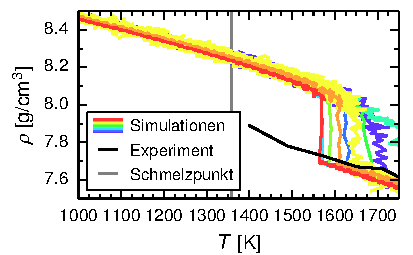
\includegraphics[width=\textwidth]{Cu_u6_meltingpoint}
    \subcaption{Phasenübergang mit Cu\_u6.eam bei unterschiedlichen $t_\text{relax}$}
  \end{subfigure}
  \hfill
  \begin{subfigure}[t]{\subfigwidth}
    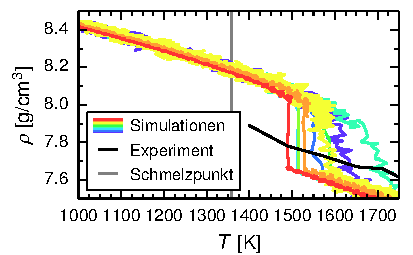
\includegraphics[width=\textwidth]{Cu_smf7_meltingpoint}
    \subcaption{Phasenübergang mit Cu\_smf7.eam bei unterschiedlichen $t_\text{relax}$}
  \end{subfigure}
  \caption[Abweichung der Schmelztemperaturen bei Kupfer-MD]{
    Abweichung der Schmelztemperatur mit verschiedenen Parametrisierungen.
    Experimentelle Werte von Brillo et al.\cite{brillo_density_2006}.
  }
  \label{fig:copperthermo}
\end{figure}

\subsection{Prozess-Simulation}
\label{coppersimulation}

\begin{figure}
  \captionsetup[subfigure]{singlelinecheck=false}
  \def\subfigwidth{0.49\textwidth}
  \begin{subfigure}[t]{\subfigwidth}
    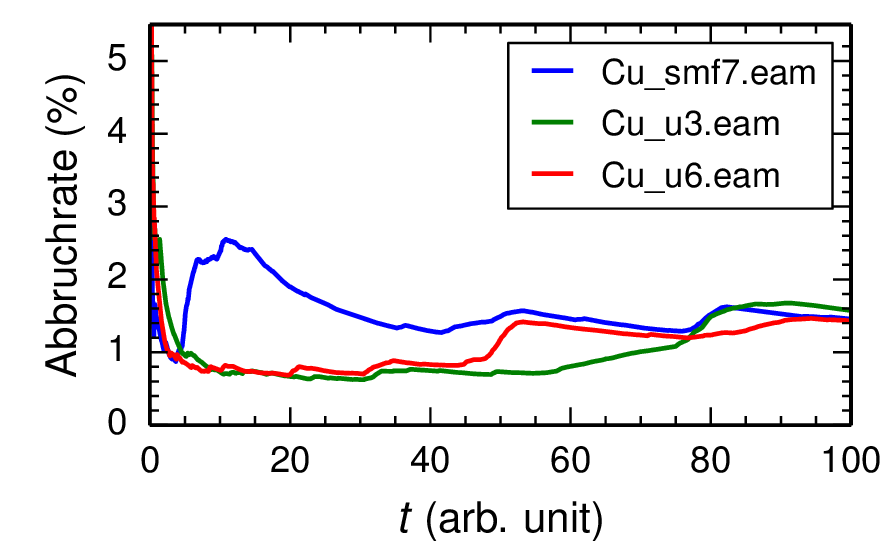
\includegraphics[width=\textwidth]{Cu_abortstatplot}
    \subcaption{Verlauf der Abbruchraten}
    \label{fig:copperparsivald-a}
  \end{subfigure}
  \hfill
  \begin{subfigure}[t]{\subfigwidth}
    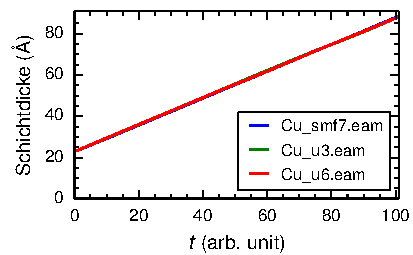
\includegraphics[width=\textwidth]{Cu_thickness}
    \subcaption{Zeitliche Entwicklung der Schichtdicke}
    \label{fig:copperparsivald-b}
  \end{subfigure}
  \begin{subfigure}[t]{\subfigwidth}
    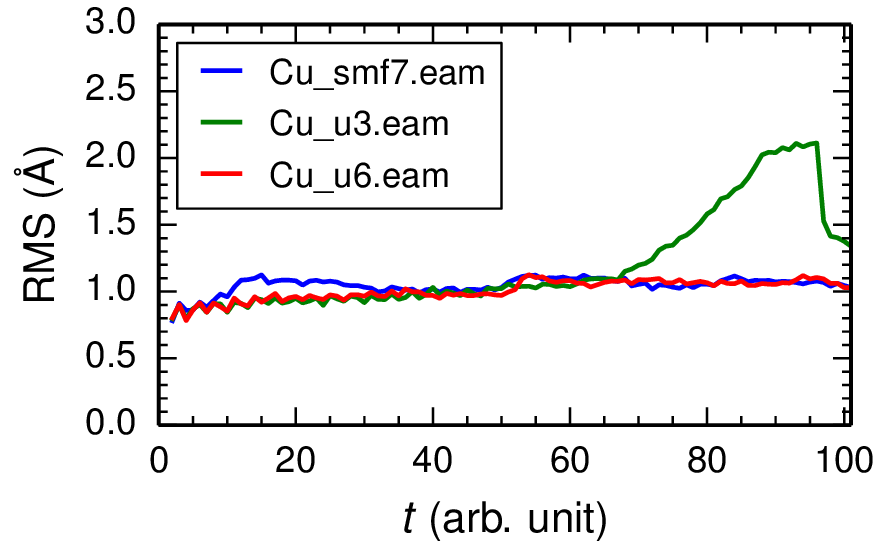
\includegraphics[width=\textwidth]{Cu_roughness}
    \subcaption{Zeitliche Entwicklung der Rauheit}
    \label{fig:copperparsivald-c}
  \end{subfigure}
  \hfill
  \begin{subfigure}[t]{\subfigwidth}
    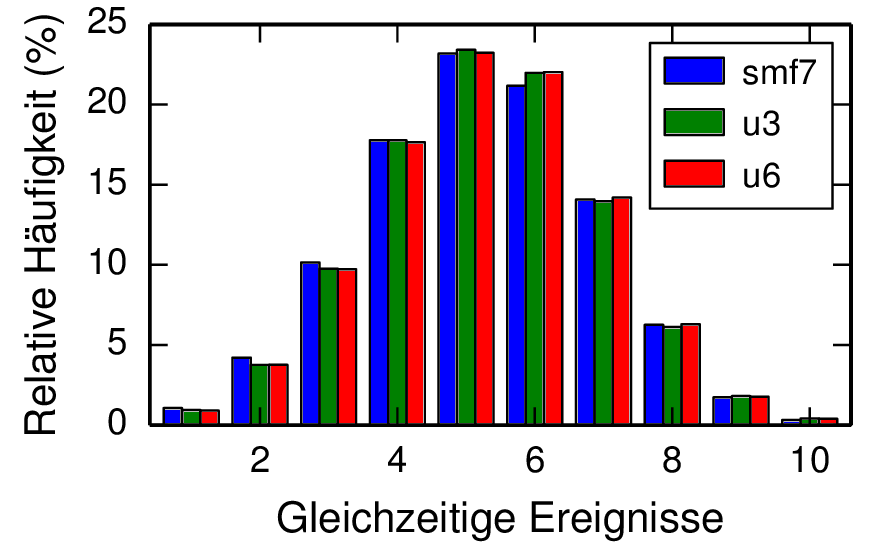
\includegraphics[width=\textwidth]{Cu_eventhistogram}
    \subcaption{Häufigkeit gleichzeitiger Ereignisse}
    \label{fig:copperparsivald-d}
  \end{subfigure}
  \caption{Vergleich der Kupfer-Potentiale in Parsivald-Rechnungen}
  \label{fig:copperparsivald}
\end{figure}

Aufgrund der Ähnlichkeit des Gold-PVD-Prozesses wurden dessen Parameter für die Kupfer-PVD übernommen und auf deren Eigenschaften angepasst.
Beispielsweise liegen kleinere Bindungslängen und geringere Massen vor, die zu erhöhten Auftreff- und geschwindigkeiten führen.

Zu Beginn der Simulation ergeben sich hohe Abbruchrate von \SI{25}{\percent}, die durch Herausschlagen einzelner Atome bei Ankunft eines neuen Kupferatomes verursacht werden.
Bereits nach wenigen Oberflächenereignissen nimmt die Abbruchrate ab, was auf eine Reduktion des Effektes durch thermische Relaxation und Bedeckung der Oberfläche durch temporäre Off-Lattice-Atome hinweist.
Die kritische Bedeckung dafür liegt zwischen \SI{0.034}{\per\nano\meter\squared} und \SI{0.074}{\per\nano\meter\squared} und deckt sich somit mit der maximalen MD-Ereignisdichte von \SI{0.073}{\per\nano\meter\squared}.
Das deutet darauf hin, dass perfekte Gitterkonfigurationen nicht robust gegenüber gerichteten Energieeinträgen ist, kleine Störungen des Gitters aber zur gleichmäßigeren Verteilung der eingebrachten Energien führen.
\todo[inline]{Entropieargument einbringen?}

Im weiteren Verlauf der Simulation variiert die Abbruchquote unterhalb von \SI{2}{\percent} (Abbildung \ref{fig:copperparsivald-a}).
Sie korreliert augenscheinlich mit der RMS-Rauheit (Abbildung \ref{fig:copperparsivald-c}), die durch Oberflächenunebenheiten auf der Nanometer-Skala dominiert wird.
Mit einem nahezu konstanten RMS-Wert um \SI{1}{\angstrom} sind die gewachsenen Schichten durchgehend glatt, mit Ausnahme des Cu\_u3.eam-Systemes.

Die Cu\_u3.eam-Simulation bildet ab Schritt 70 einen \SI{2.6}{\nano\meter} breiten und \SI{3.0}{\nano\meter} tiefen \todo{Krater?}Krater aus, der schließlich zu einem \SI{1}{\nano\meter} großen \todo{void}Einschluss abgeschlossen wird (Abbildung \ref{fig:coppercrater}).
Die Auswirkungen dieses Kraters sind auch im RMS-Diagramm (Abbildung \ref{fig:copperparsivald-c}, schlagartige Abnahme in Schritt 96) und in den Abbruchraten (Abbildung \ref{fig:copperparsivald-a}, Anstieg zwischen Schritten 60 und 90) erkennbar, beeinflussen aber nicht die Wachstumsrate (Abbildung \ref{fig:copperparsivald-b}).

\begin{figure}

  \captionsetup[subfigure]{justification=centering,singlelinecheck=false}
  \def\subfigwidth{0.32\textwidth}

  \begin{subfigure}[t]{\subfigwidth}
    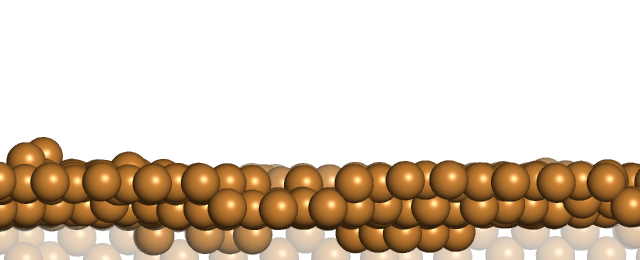
\includegraphics[width=\textwidth]{Cu_crater_01_crop}
    \subcaption{$t=59$}
  \end{subfigure}
  \hfill
  \begin{subfigure}[t]{\subfigwidth}
    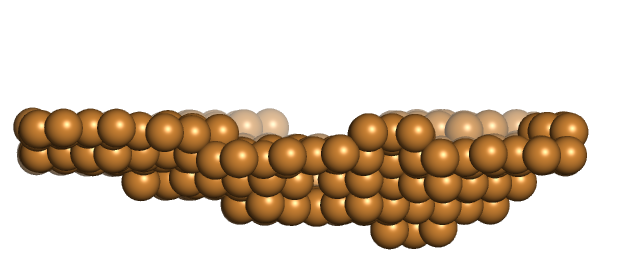
\includegraphics[width=\textwidth]{Cu_crater_07_crop}
    \subcaption{$t=65$}
  \end{subfigure}
  \hfill
  \begin{subfigure}[t]{\subfigwidth}
    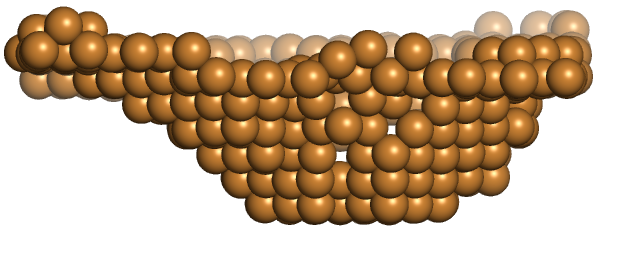
\includegraphics[width=\textwidth]{Cu_crater_17_crop}
    \subcaption{$t=75$}
  \end{subfigure}

  \begin{subfigure}[t]{\subfigwidth}
    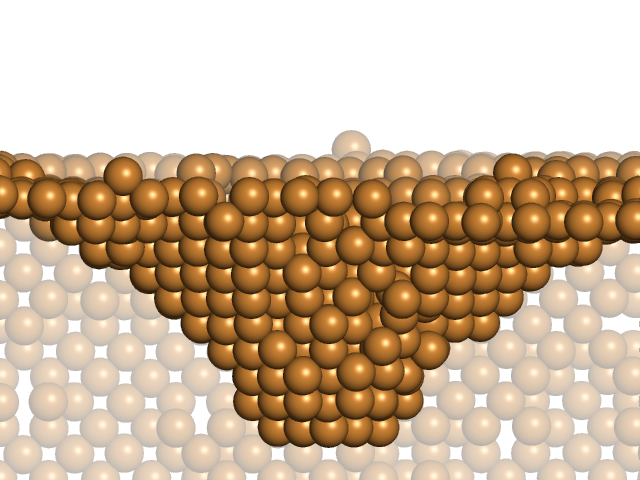
\includegraphics[width=\textwidth]{Cu_crater_27}
    \subcaption{$t=85$}
  \end{subfigure}
  \hfill
  \begin{subfigure}[t]{\subfigwidth}
    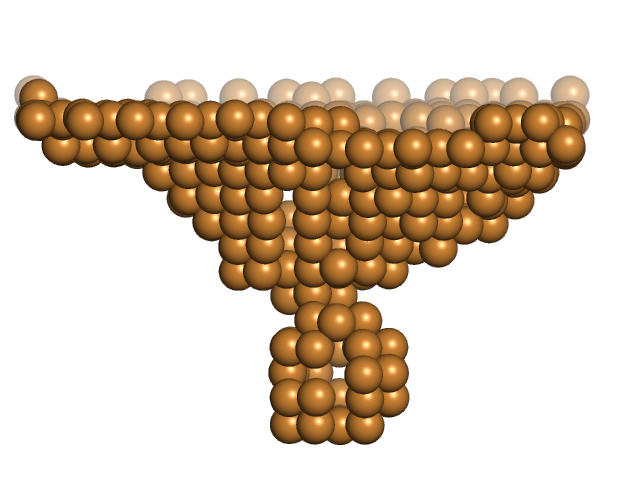
\includegraphics[width=\textwidth]{Cu_crater_37}
    \subcaption{$t=95$}
  \end{subfigure}
  \hfill
  \begin{subfigure}[t]{\subfigwidth}
    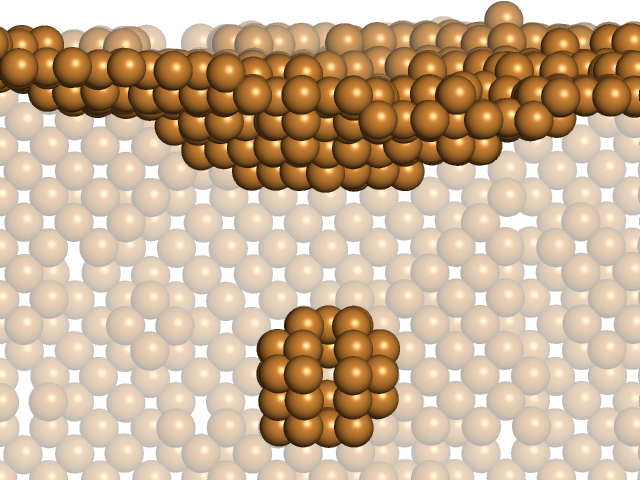
\includegraphics[width=\textwidth]{Cu_crater_42}
    \subcaption{$t=100$}
  \end{subfigure}

  \caption{Wachstum und Abschluss des Kupfer-Kraters bei Cu\_u3.eam.\\
    Seitenansicht der extrahierten Oberflächenatome (\SI{3x3}{\nano\meter})
  }
  \label{fig:coppercrater}
\end{figure}

\subsubsection{Maximale Ereignisdichte}
Ergänzend ist in Abbildung \ref{fig:copperparsivald-d} ein Histogramm der Zahl paralleler Ereignisse dargestellt.
Die maximale Oberflächendichte der Ereignisse liegt bei der gewählten MD-Box-Größe von \SI{37x37}{\angstrom} bei \SI{0.073}{\per\nano\meter\squared}.
Dem stehen beobachtete Werte von 12 aktiven Ereignissen gegenüber, die einer Dichte von \SI{0.03}{\per\nano\meter\squared} und somit \SI{40}{\percent} maximaler Bedeckung entsprechen.
Aufgrund der zufälligen Positionierung der MD-Box innerhalb der KMC-Simulation und der Blocking von Ereignissen bei Überlappung der MD-Kästen scheint dieser Wert plausibel.
Ähnliche Werte werden bei Simulationsläufen mit unterschiedlichen Substratgrößen und Materialien beobachtet werden.
